\documentclass[letterpaper,12pt]{article}
\usepackage{array}
\usepackage{threeparttable}
\usepackage{geometry}
\usepackage{amsmath}
\geometry{letterpaper,tmargin=1in,bmargin=1in,lmargin=1.25in,rmargin=1.25in}
\usepackage{fancyhdr,lastpage}
\pagestyle{fancy}
\lhead{}
\chead{}
\rhead{}
\lfoot{}
\cfoot{}
\rfoot{\footnotesize\textsl{Page \thepage\ of \pageref{LastPage}}}
\renewcommand\headrulewidth{0pt}
\renewcommand\footrulewidth{0pt}
\usepackage[format=hang,font=normalsize,labelfont=bf]{caption}
\usepackage{listings}
\lstset{frame=single,
  language=Python,
  showstringspaces=false,
  columns=flexible,
  basicstyle={\small\ttfamily},
  numbers=none,
  breaklines=true,
  breakatwhitespace=true
  tabsize=3
}
\usepackage{amsmath}
\usepackage{amssymb}
\usepackage{amsthm}
\usepackage{harvard}
\usepackage{setspace}
\usepackage{float,color}
\usepackage[pdftex]{graphicx}
\usepackage{hyperref}
\hypersetup{colorlinks,linkcolor=red,urlcolor=blue}
\theoremstyle{definition}
\newtheorem{theorem}{Theorem}
\newtheorem{acknowledgement}[theorem]{Acknowledgement}
\newtheorem{algorithm}[theorem]{Algorithm}
\newtheorem{axiom}[theorem]{Axiom}
\newtheorem{case}[theorem]{Case}
\newtheorem{claim}[theorem]{Claim}
\newtheorem{conclusion}[theorem]{Conclusion}
\newtheorem{condition}[theorem]{Condition}
\newtheorem{conjecture}[theorem]{Conjecture}
\newtheorem{corollary}[theorem]{Corollary}
\newtheorem{criterion}[theorem]{Criterion}
\newtheorem{definition}[theorem]{Definition}
\newtheorem{derivation}{Derivation} % Number derivations on their own
\newtheorem{example}[theorem]{Example}
\newtheorem{exercise}[theorem]{Exercise}
\newtheorem{lemma}[theorem]{Lemma}
\newtheorem{notation}[theorem]{Notation}
\newtheorem{problem}[theorem]{Problem}
\newtheorem{proposition}{Proposition} % Number propositions on their own
\newtheorem{remark}[theorem]{Remark}
\newtheorem{solution}[theorem]{Solution}
\newtheorem{summary}[theorem]{Summary}
%\numberwithin{equation}{section}
\bibliographystyle{aer}
\newcommand\ve{\varepsilon}
\newcommand\boldline{\arrayrulewidth{1pt}\hline}


\begin{document}

\begin{flushleft}
  \textbf{\large{Problem Set \#2}} \\
  MACS 30100, Dr. Evans \\
  Soo Wan Kim
\end{flushleft}

\noindent\textbf{Problem 1} \\
\textbf {Part (a)}

\begin{figure}[h!]
  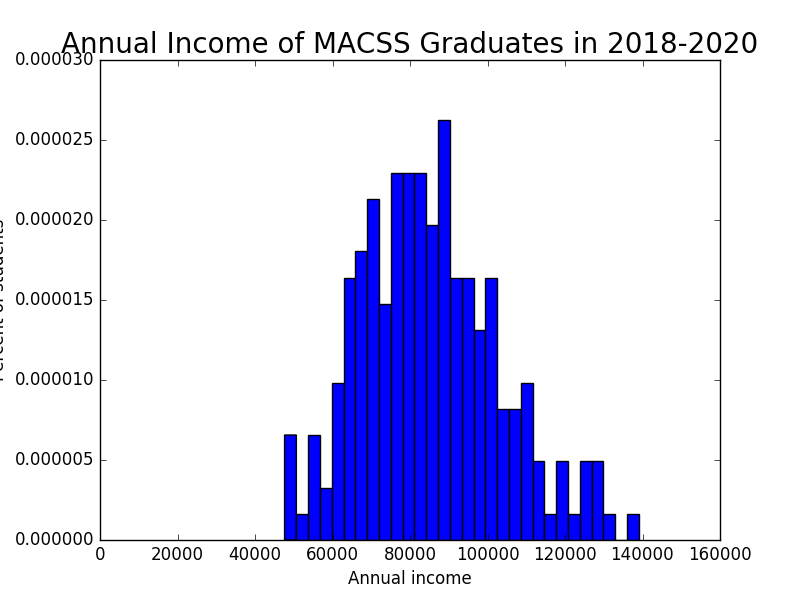
\includegraphics[width=\linewidth]{1a.png}
  \caption{Histogram of percentages of the income.text data}
\end{figure}

\noindent
\textbf {Part (b)} 

\begin{figure}[h!]
  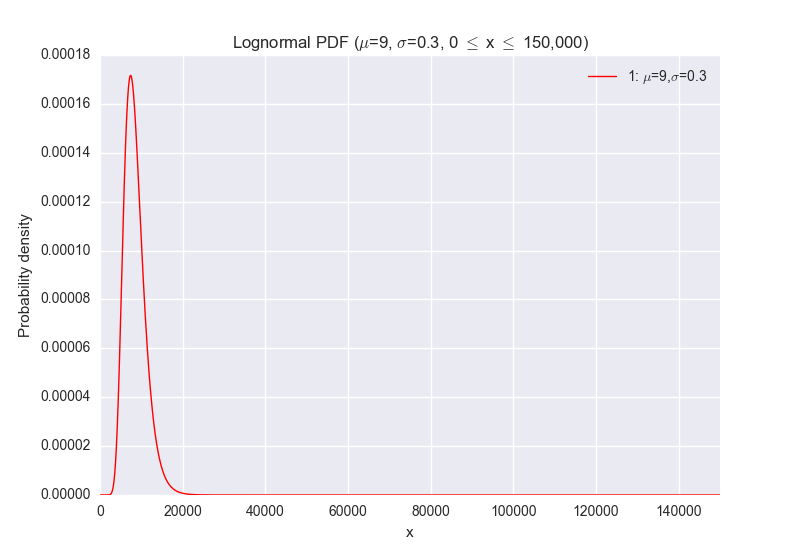
\includegraphics[width=\linewidth]{1b.png}
  \caption{Lognormal PDF with $\mu$ = 9.0 and $\sigma$ = 0.3}
\end{figure}

\noindent
Log likelihood value: -8298.63695601\\

\noindent\textbf {Part (c).} 

\begin{figure}[h!]
  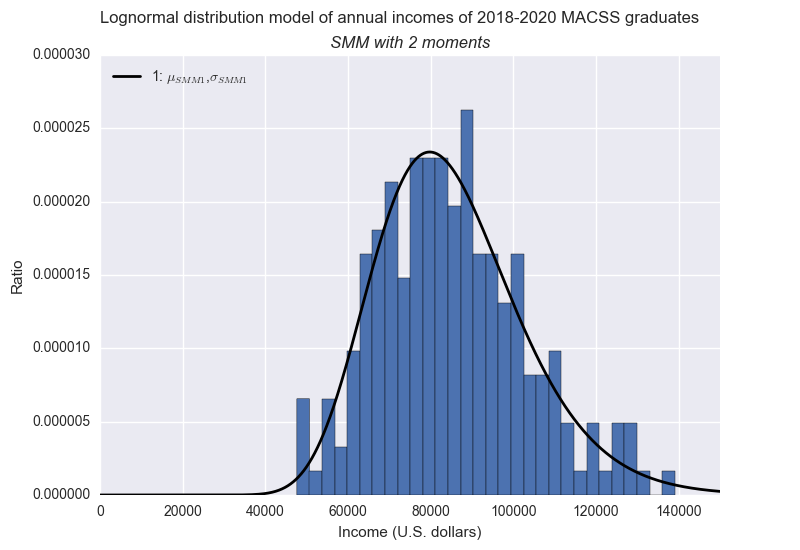
\includegraphics[width=\linewidth]{1c.png}
  \caption{Lognormal PDF with MLE estimates for $\mu$ and $\sigma$}
\end{figure}

\noindent
$\mu$ MLE = 11.3314411636\\
$\sigma$ MLE = 0.211674565363 \\\\
Log likelihood value: -2239.534744\\
Variance-covariance matrix: \\
$$ \left[
\begin{array}{c c}
2.22922149e-04 		& 		9.27073415e-06 \\
9.27073415e-06 		& 		1.64466141e-04 \\
\end{array} \right] 
$$

\noindent\textbf {Part (d).} \\
The probability that the incomes data has $\mu$ = 9.0 and $\sigma$ = 0.3 is 0. \\

\noindent
\textbf {Part (e).} \\
The probability that I will learn more than \$100,000 is: 0.195766989696 \\
The probability that I will learn less than \$75,000 is: 0.307687164314\\

\noindent\textbf{Problem 2} \\
\textbf {Part (a).} \\\\
\noindent
$\beta_0$ MLE = 0.293418697526\\
$\beta_1$ MLE = 0.00763476963395\\
$\beta_2$ MLE = 0.444707732948\\
$\beta_3$ MLE = -0.00780350965027\\
$\sigma$ MLE = 0.0230457171774\\\\
Log likelihood value: 477.537339914\\
Variance-covariance matrix: \\
$$ \left[
\begin{array}{ccccc}
 1 & 0 & 0 & 0 & 0 \\
 0 & 1 & 0 & 0 & 0 \\
 0 & 0 & 1 & 0 & 0 \\
 0 & 0 & 0 & 1 & 0 \\
 0 & 0 & 0 & 0 & 1 \\
\end{array} \right] 
$$

\noindent
\textbf {Part (b).} \\
\noindent
The probability that $\beta_0$ = 1.0, $\sigma^2$ = 0.01, and $\beta_1$, $\beta_2$, $\beta_3$ = 0 is 0.  \\



\end{document}
